\documentclass{article}
\usepackage{fullpage}
\usepackage{multicol,multirow}
\usepackage{tabularx}
\usepackage{ulem}
\usepackage[utf8]{inputenc}
\usepackage[russian]{babel}
\usepackage{pgfplots}
\usepackage{graphicx}

\begin{document}

\section*{Курсовая работа по курсу «Численные методы»}
\section*{Решение краевых задач для нелинейных дифференциальных уравнений 
методом конечных разностей}

Выполнил студент группы М8О-408Б-20 Попов Матвей.
\\
Преподаватель: Пивоваров Д.\,Е.

\subsection*{Цель}

Реализовать решение краевых задач для нелинейных дифференциальных уравнений 
второго порядка методом конечных разностей. То есть, найти решение ДУ вида 
$$F(x, y, y', y'') = 0$$
на отрезке $[a, b]$ при краевых условиях
$$a_1 y(a) + b_1 y'(a) = c_1$$
$$a_1 y(b) + b_1 y'(b) = c_2$$
где $|a_1| + |b_1| > 0$ и $|a_2| + |b_2| > 0$.

\subsection*{Тесты}
$$y'' + 4xy' + (4x^2 + 2)y = 0$$
$$y'(0) = 1$$
$$4y(2) - y'(2) = 23e^{-4}$$
Аналитическое решение:
$$y(x) = (1 + x)e^{-x^2}$$

\subsection*{О программе}
Программа написана на Python 3.8. Реализации всех методов находятся в папке 
app.

\subsection*{Инструкция к запуску}
\texttt{pip3 install -r requirements.txt}\\
\texttt{python3 main.py}\\

\subsection*{Результаты}
\begin{center}
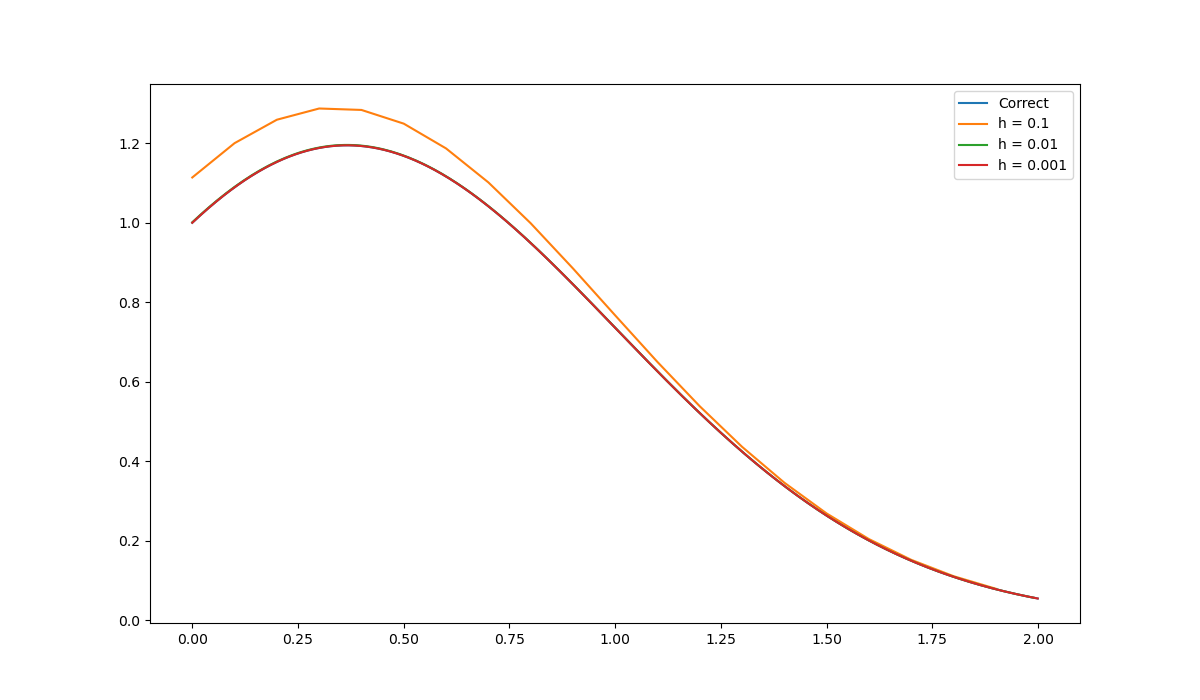
\includegraphics[scale=0.25]{img/img01.png}
\end{center}


\subsection*{Вывод}
Проделав лабораторную работу, я решил краевую задачу для нелинейных ДУ 
методом конечных разностей и проверил погрешности полученных вычислений.

\end{document}
